\documentclass[conference]{IEEEtran}

\usepackage{url}
\usepackage{graphicx}
\usepackage{caption}
\usepackage{subcaption}
\usepackage{hyperref}
\usepackage{url}
\usepackage{times}
\usepackage{balance}
\usepackage{xspace}
\usepackage{paralist}
\usepackage{color}
\usepackage{amssymb}

\clubpenalty = 10000
\widowpenalty = 10000
\displaywidowpenalty = 10000

\begin{document}

\newcommand{\ghtorrent}{\textsc{ght}orrent\xspace}
\newcommand{\prioritizer}{\textsc{pr}ioritizer\xspace}
\newcommand{\api}{\textsc{api}\xspace}
\newcommand{\todo}[1]{\textcolor{red}{\textbf{\textsc{todo:}} #1}}

\newcommand{\nb}[3]{
  \fcolorbox{black}{#2}{\bfseries\sffamily\scriptsize#1}
    {\sf\small$\blacktriangleright$\textit{#3}$\blacktriangleleft$}
}

\newcommand\georgios[1]{\nb{Georgios}{yellow}{#1}}
\newcommand\andy[1]{\nb{Andy}{cyan}{#1}}
\newcommand\erik[1]{\nb{Erik}{magenta}{#1}}

\newcommand{\hassanbox}[1]
{
  \vspace{0.29em}
  \noindent
  \fbox{
  \begin{minipage}{0.46\textwidth}
    \emph{\noindent #1}
    \end{minipage}
}}

% Macros for qualitative research :-)
\newcommand{\resp}[2]{{\sc R#1:} ``\emph{#2}''}
\newcommand{\respnum}[1]{{\sc R#1}}
\newcommand{\code}[1]{{\textsl{#1}}}

\title{Pull Request Prioritization}


\author{\IEEEauthorblockN{Erik van der Veen, Georgios Gousios, Andy Zaidman}
\IEEEauthorblockA{Delft University of Technology,\\The Netherlands}
\IEEEauthorblockA{\{e.v.d.veen@tudelft.nl, g.gousios, a.e.zaidman\}@tudelft.nl}
}


\author{\IEEEauthorblockN{Erik van der Veen}
\IEEEauthorblockA{Delft University of Technology\\
the Netherlands\\
Email: e.v.d.veen@tudelft.nl}
\and
\IEEEauthorblockN{Georgios Gousios}
\IEEEauthorblockA{Radboud University Nijmegen\\
the Netherlands\\
Email:georgios@cs.ru.nl}
\and
\IEEEauthorblockN{Andy Zaidman}
\IEEEauthorblockA{Delft University of Technology\\
the Netherlands\\
Email: a.e.zaidman@tudelft.nl}}

\maketitle

\begin{abstract}

\end{abstract}

%\category{D.2.7}{Software Engineering}{Distribution, Maintenance, and Enhancement}[Version control]
%\category{D.2.9}{Software Engineering}{Management}[Programming teams]

%\terms{Management}

%\keywords{pull-based development, pull request, distributed software development,
%empirical software engineering}

\section{Introduction}

Pull-based development as a distributed development model is a distinct way of
collaborating in software development. In this model, the project's main
repository is not shared among potential contributors; instead, contributors
fork (clone) the repository and make their changes independent of each other.
When a set of changes is ready to be submitted to the main repository, they
create a pull request, which specifies a local branch to be merged with a branch
in the main repository. A member of the project's core team (the
\emph{integrator}) is responsible to inspect the changes and integrate them into
the project's main development line.

In earlier work~\cite{GZSD15}, we surveyed 750 pull request integrators from high
volume projects and discovered that the top two challenges they face when
working with pull requests are maintaining project quality and prioritizing work
in the face of multiple concurrent pull requests. With respect to pull request
prioritization our findings are summarized in Figure~\ref{fig:prioritization}.

In this paper, we present the design and initial implementation of a prototype
pull request prioritization tool, the \prioritizer. \prioritizer works as a
priority inbox for pull requests: it examines all open pull requests and
presents to project integrator the top 5 pull requests that need their immediate
attention. It also offers an alternative view to Github's pull request
interface, which allows developers to sort open pull requests on a multitude of
criteria, ranging from the pull request's age to its number of pairwise
conflicts. \prioritizer is a service-oriented architecture build on top of
\ghtorrent: it uses \ghtorrent's data collection mechanisms to react in near
real-time to changes to pull request state and databases as a source of easy to
access metadata.


\begin{figure}[t]
  \begin{center}
    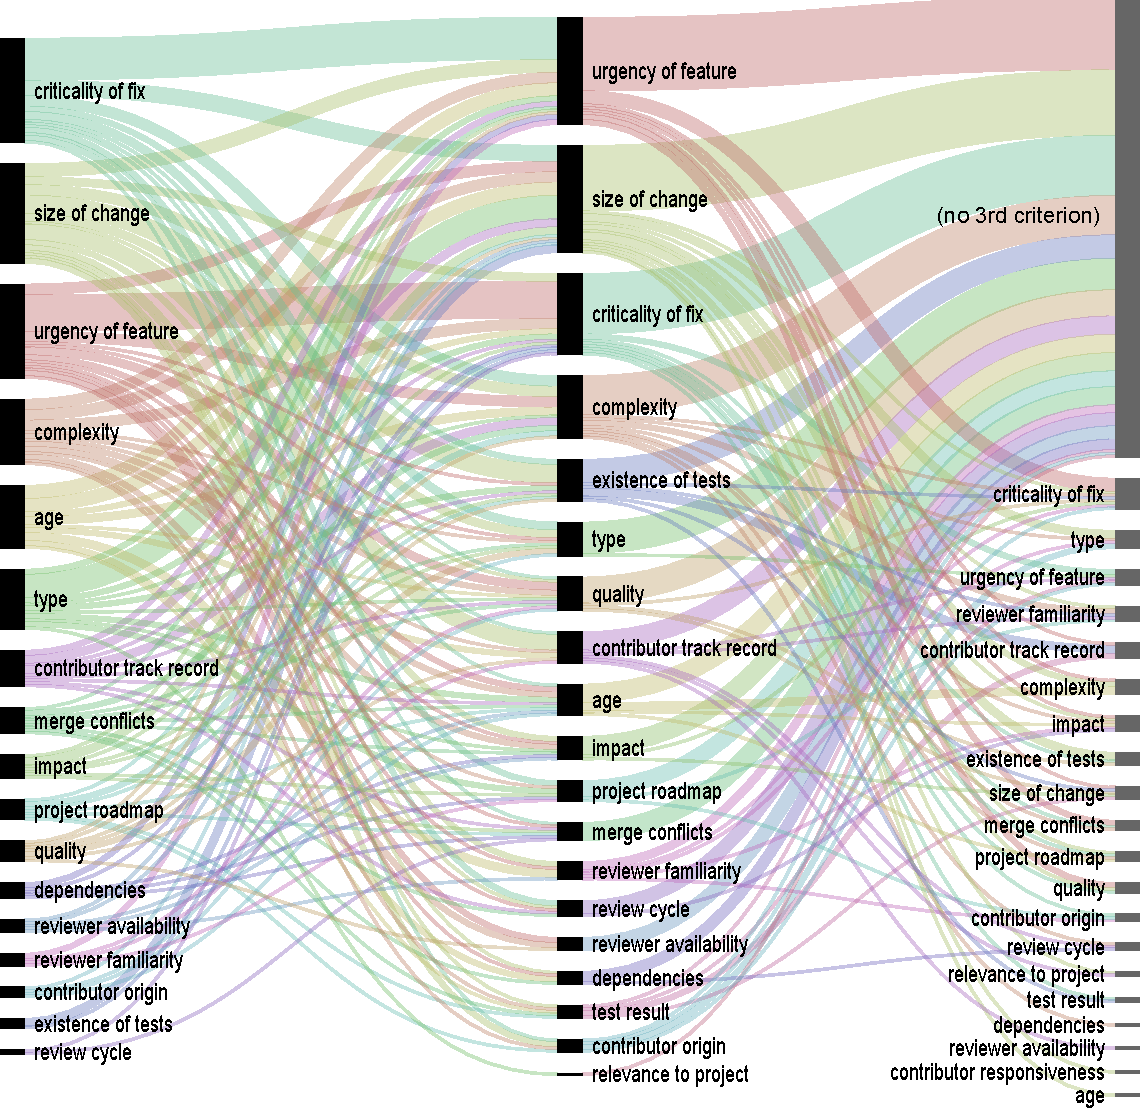
\includegraphics[scale=0.44]{prioritization-criteria}
  \end{center}
  \caption{Prioritization criteria and their order of application as reported by
  750 integrators.}
  \label{fig:prioritization}
\end{figure}


\section{Prioritizing pull requests}

\subsection{Modeling} Contrary to common approaches to work prioritization, which usually produce
an optimal ordering for open work items based on optimization processes, we
modelled the pull request prioritization using the priority inbox approach.
What \prioritizer tries to do is present the integrators with the 3 pull
requests that will need their immediate attention. \andy{Need some related
work support here}

To select the important pull requests, \prioritizer uses machine learning.
Initially, time is split in configurable time windows (currently, 1 day long).
In each time window, it calculates a list of features for all pull requests
(dependent variables, explained below) and a boolean response variable that
indicates whether the received a user action in the following time window. A
machine learning algorithm is then applied on historical data to build a model
for predicting whether current pull requests will receive user updates in the
following time window. The 3 pull requests with the highest probability to be
updated are classified as the important ones. \erik{Please check what I write
here is correct}.

\subsection{Features}
Our feature set was extracted by analysing the results of the survey and
closely correspond to the developer's answers are reported in
Figure~\ref{fig:prioritization}. An overview of the selected features can
be seen in Table~\ref{tab:features}.

\begin{table*}[ht]
  \centering
  \begin{tabular}{rp{26em}rrrrc}
    \hline
    \textbf{Feature} & \textbf{Description} & \textbf{5\%} & \textbf{Mean} & \textbf{Median} & \textbf{95\%} & \textbf{Plot} \\
    \hline
    Age & Minutes between open and the current time window start time. & 0.00 & 167344.02 & 77760.00 & 646560.00 & 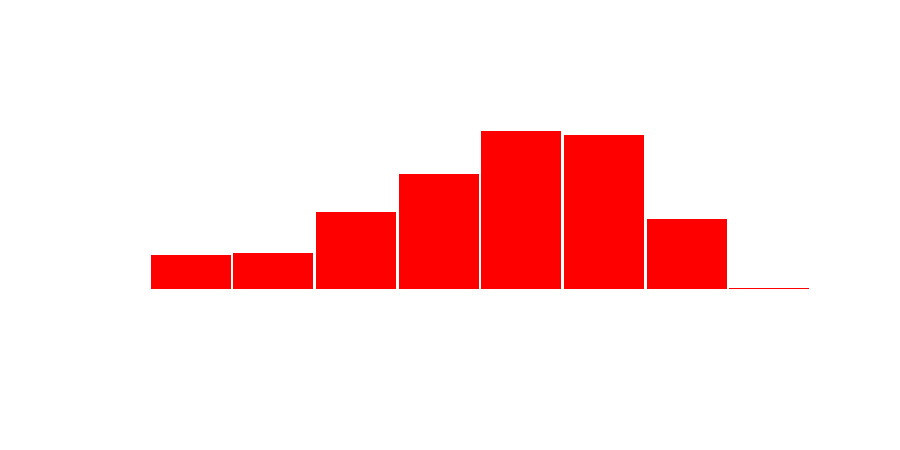
\includegraphics[scale = 0.1, clip = true, trim= 50px 60px 50px 60px]{../figs/hist-features/hist-age.pdf} \\
    Contribution Rate & The percentage of commits by the author currently in the project. & 0.00 & 0.03 & 0.00 & 0.14 & 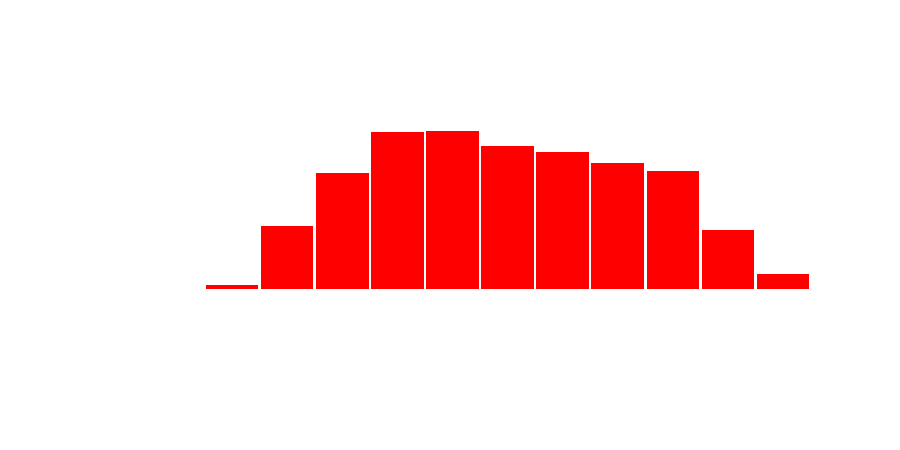
\includegraphics[scale = 0.1, clip = true, trim= 50px 60px 50px 60px]{../figs/hist-features/hist-commitRatio.pdf} \\
    Accept Rate & The percentage of the author's other PRs that have been merged. & 0.00 & 0.45 & 0.50 & 0.90 & 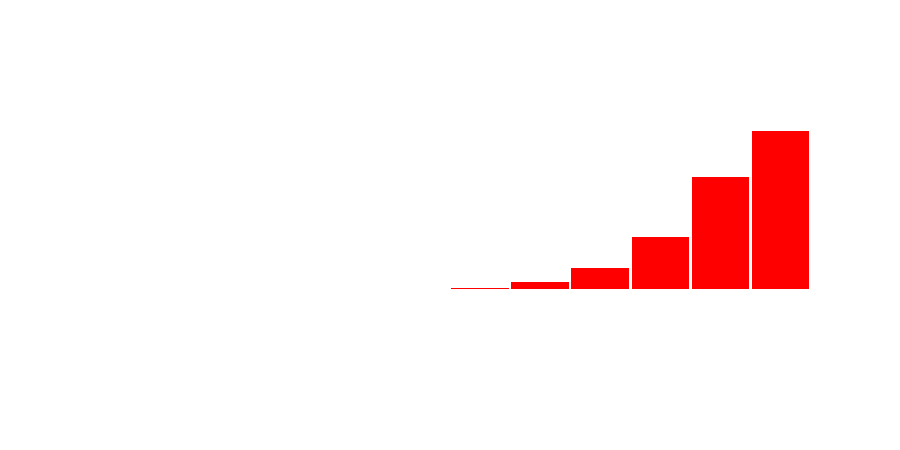
\includegraphics[scale = 0.1, clip = true, trim= 50px 60px 50px 60px]{../figs/hist-features/hist-pullRequestRatio.pdf} \\
    Additions & Number of lines added. & 1.00 & 3649.86 & 41.00 & 6285.00 & 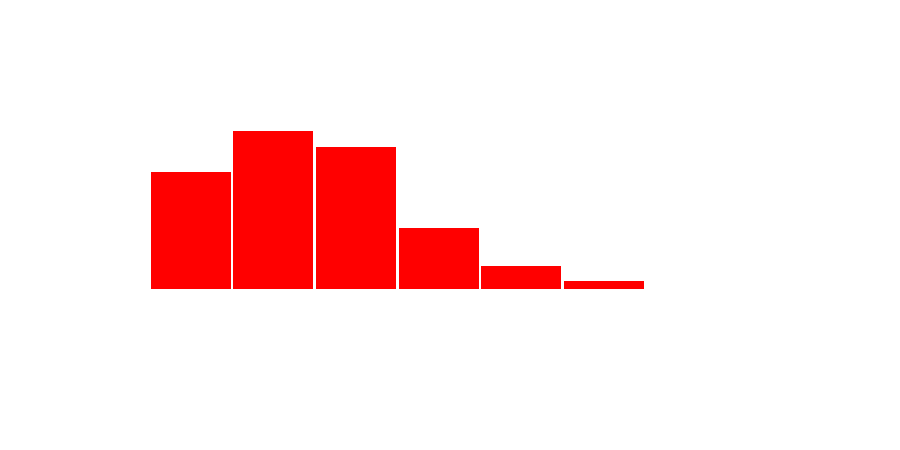
\includegraphics[scale = 0.1, clip = true, trim= 50px 60px 50px 60px]{../figs/hist-features/hist-additions.pdf} \\
    Deletions & Number of lines deleted. & 0.00 & 2271.32 & 7.00 & 2353.00 & 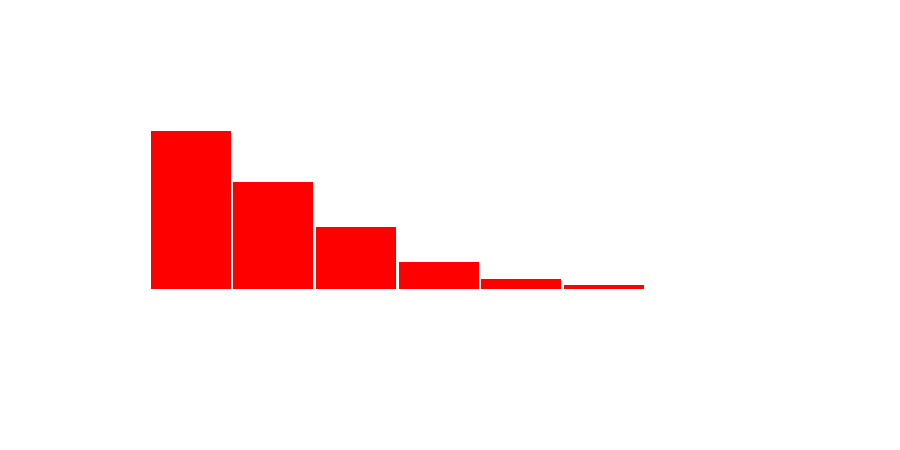
\includegraphics[scale = 0.1, clip = true, trim= 50px 60px 50px 60px]{../figs/hist-features/hist-deletions.pdf} \\
    Commits & Number of commits. & 1.00 & 6.52 & 2.00 & 22.00 & 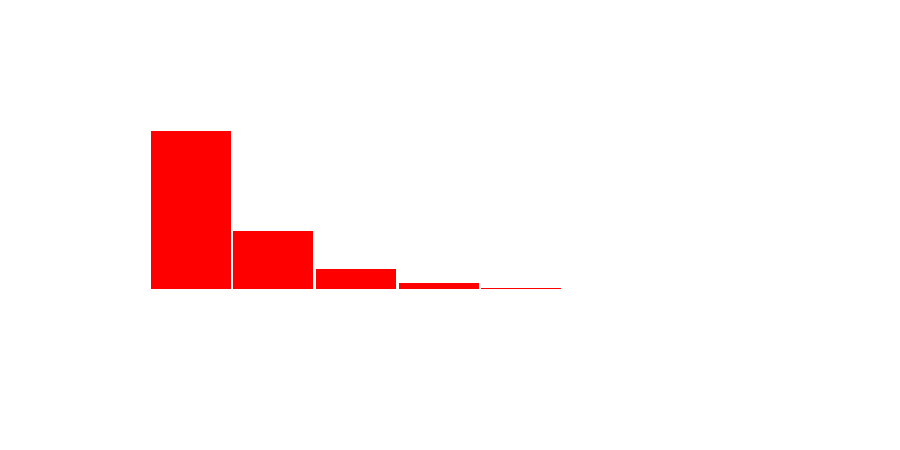
\includegraphics[scale = 0.1, clip = true, trim= 50px 60px 50px 60px]{../figs/hist-features/hist-commits.pdf} \\
    Files & Number of files touched. & 1.00 & 53.88 & 2.00 & 125.00 & 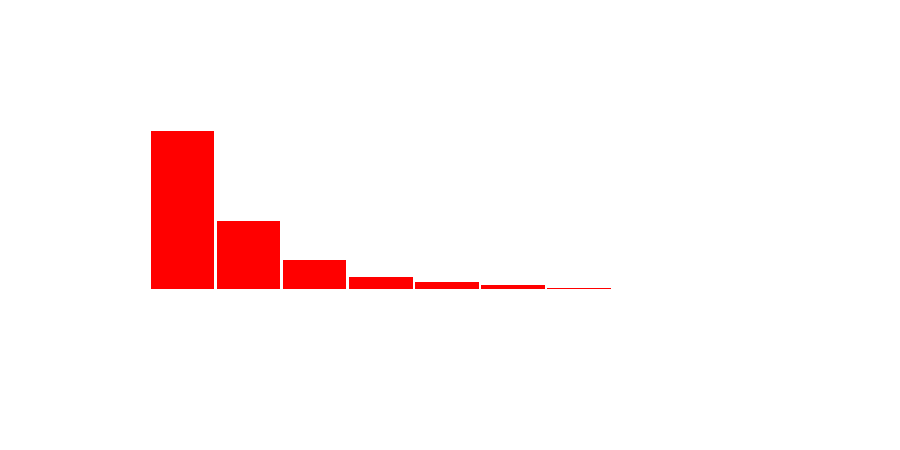
\includegraphics[scale = 0.1, clip = true, trim= 50px 60px 50px 60px]{../figs/hist-features/hist-files.pdf} \\
    Comments & Number of discussion comments. & 0.00 & 4.22 & 1.00 & 17.00 & 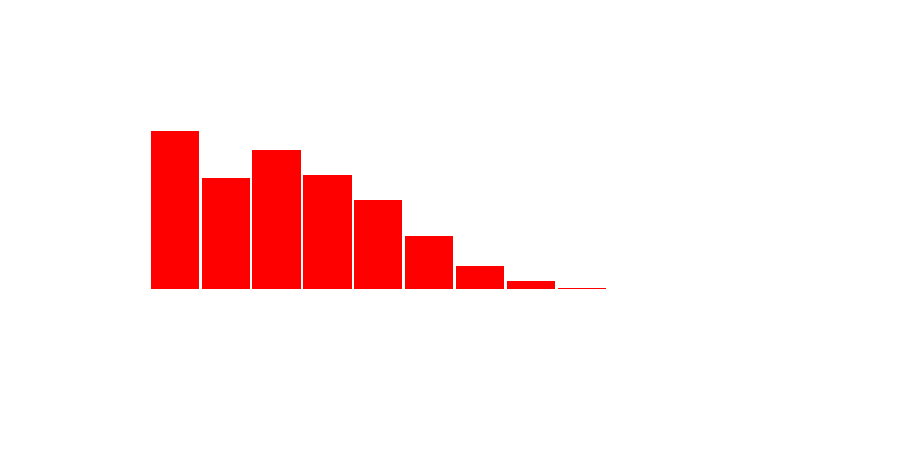
\includegraphics[scale = 0.1, clip = true, trim= 50px 60px 50px 60px]{../figs/hist-features/hist-comments.pdf} \\
    Review Comments & Number of code review comments. & 0.00 & 1.60 & 0.00 & 8.00 & 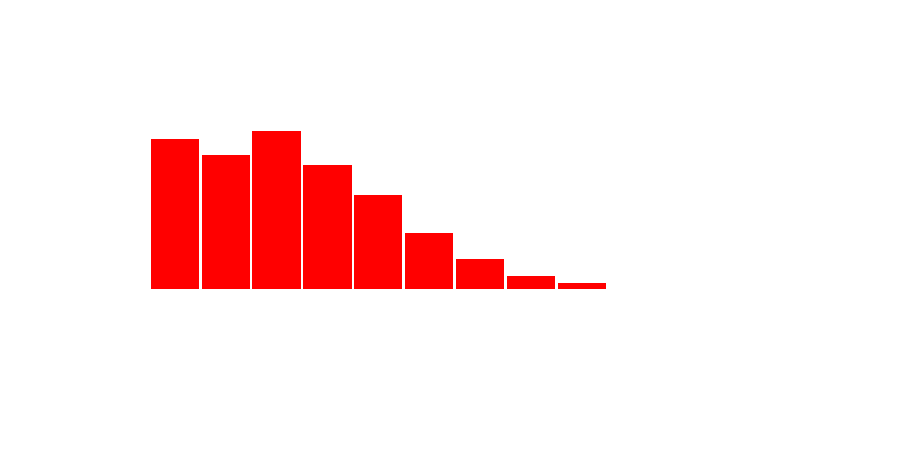
\includegraphics[scale = 0.1, clip = true, trim= 50px 60px 50px 60px]{../figs/hist-features/hist-reviewComments.pdf} \\
    Core Member & Is the author a project member? & 0.00 & 0.26 & 0.00 & 1.00 & 
\includegraphics[scale = 0.1, clip = true, trim= 50px 60px 50px 60px]{../figs/hist-features/hist-coreMember.pdf} \\
    Intra-Branch & Are the source and target repositories the same? & 0.00 & 0.06 & 0.00 & 1.00 & 
\includegraphics[scale = 0.1, clip = true, trim= 50px 60px 50px 60px]{../figs/hist-features/hist-intraBranch.pdf} \\
    Contains Fix & Is the pull request an issue fix? & 0.00 & 0.18 & 0.00 & 1.00 & 
\includegraphics[scale = 0.1, clip = true, trim= 50px 60px 50px 60px]{../figs/hist-features/hist-containsFix.pdf} \\
    Last Comment Mention & Does the last comment contain a user mention? & 0.00 & 0.11 & 0.00 & 1.00 & 
\includegraphics[scale = 0.1, clip = true, trim= 50px 60px 50px 60px]{../figs/hist-features/hist-lastCommentMention.pdf} \\
    Has Test Code & Are tests included? & 0.00 & 0.35 & 0.00 & 1.00 & 
\includegraphics[scale = 0.1, clip = true, trim= 50px 60px 50px 60px]{../figs/hist-features/hist-hasTestCode.pdf} \\
%    Target Branch & The name of the target branch. & - & - & - & - & \\
%    Pairwise Conflicts & The number of pairwise conflicts with other PRs. & - & - & - & - & \\
    \hline
  \end{tabular}
  \caption{Selected features and descriptive statistics for predicting pull
  request activity. The calculation unit is a pull request.
  Histograms (red) are in log scale.}
  \label{tab:features}
\end{table*}


One of the top parameters that developers examine when prioritizing is the
\textsl{size of change}. We therefore include 4 related features in our
model, namely additions, deletions, commits and files.
Developers also deem the \textsl{age} of the pull request important: we measure
it within the examined time window as the elapsed time between the time window
start and the pull request creation.
\erik{please indicate HOW we calculate the most important of the remaining
features (NOT how difficult it is to calculate them :))}

The \textsl{contributor's track record} is also taken into account by
integrators. To approximate the track record, we use three features: if the
contributor is a core member, we expect his/her pull requests to take precede
contribution rate, accept rate. The value of these feature may vary a lot
between different projects. There are integrators that look at PRs of known or
trusted contributers first, their code is of known quality and often easier to
review. On the other hand there are also integrators that value PRs of new
contributors more than those of known contributers. The rationale behind this is
that new contributers are feeling more valued when they receive a fast response
on their PR. Possibly will that feeling encourage them to continue to contribute
to the project. The accept rate feature suffers possibly from accuracy problems,
as it is difficult to determine whether a PR is actually merged or not. A pull
request can be merged in different ways [3]. Merges performed via the GitHub
interface are easy to detect, but a PR which is squashed to one commit before it
is merged is difficult to detect.  As second prioritization criteria the
existence of tests emerges as an important feature. Some projects have a ex-
tensive test suite. In these projects it is often expected that new PRs contain
tests for the code they add. The heuristic used for the test code detection is
very trivial, the value of the feature is true if the PR changes at least one
file with “test” or “spec” in its file name.

\section{Design and Implementation}
\label{sec:design}


\begin{figure}
  \centering
  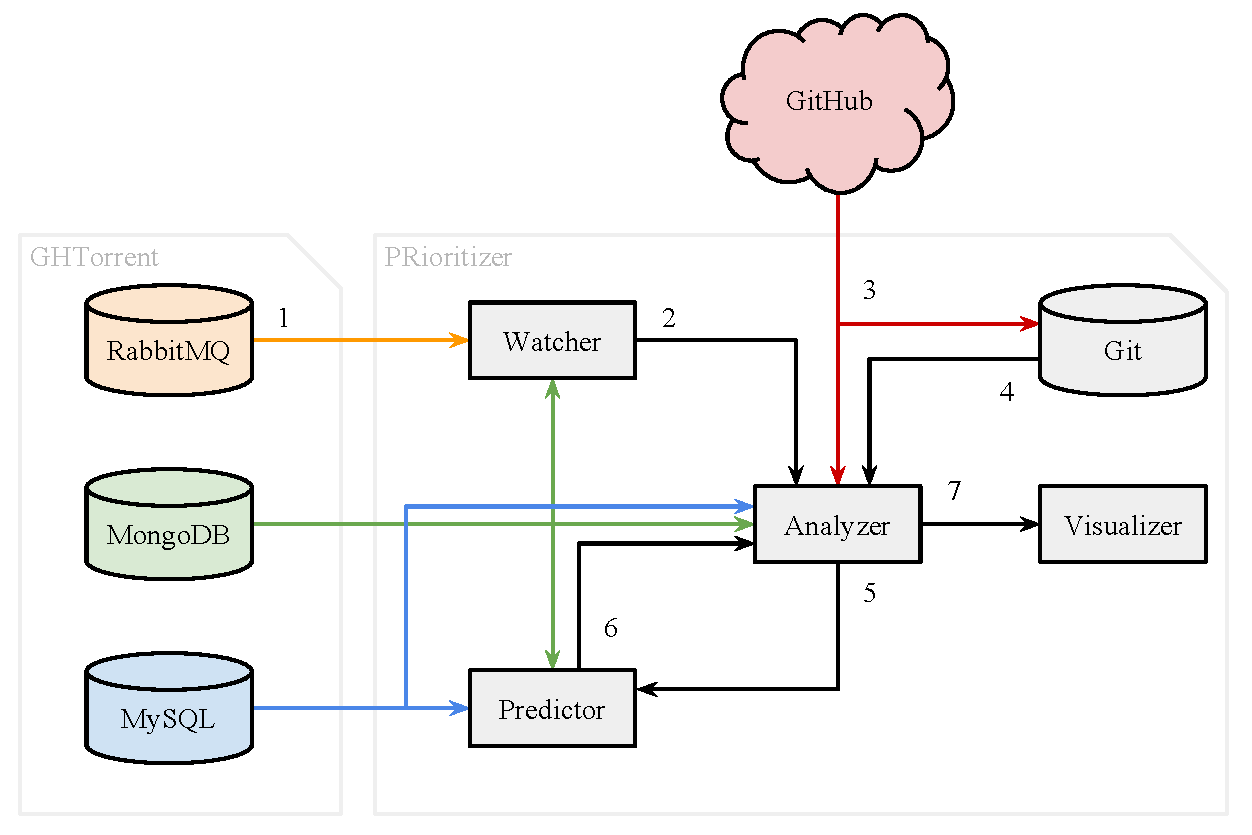
\includegraphics[width=0.5\textwidth]{../figs/architecture.pdf}
  \caption[Diagram of the architecture]
   {Diagram of the architecture. It shows the different data sources and components used by the \prioritizer service.}
  \label{fig:architecture}
\end{figure}

At its core, \prioritizer uses machine learning to predict whether a pull
request will become active within a given time frame. Excluding the repository
mining aspect, which \prioritizer uses to retrieve inputs for its prediction
engine, our goal is to build a highly scalable service, able to support any
number of repositories. We therefore designed \prioritizer as a loosely-coupled
architecture based on independent micro services. The overall architecture can be
seen in Figure~\ref{fig:architecture}. Below, we present brief descriptions
of the components comprising the \prioritizer.

\paragraph{GHTorrent}
\ghtorrent~\ref{G13} mirrors all data exposed from the GitHub \api in
real time. As such, it maintains 2 databases, an unstructured one (MongDB)
which contains the raw replies from the GitHub \api and a relational one
(MySQL) which stores indexed historical data for all GitHub repositories.
To keep track of what is happening on GitHub, is monitors the GitHub event
timeline \api endpoint and publishes the retrieved data to a queue service
(RabbitMQ) where multiple clients can connect to.
\prioritizer uses \ghtorrent as both a data source of historical data and a
source for live data.
The live data that the \prioritizer is interested in are events on pull requests triggered by actions such as assignment of the pull request to a specific
user or merging the pull request.

\paragraph{Watcher}
The watcher continuously listens to pull request event from \ghtorrent
via a RabbitMQ message queue. It maintains a list of registered repositories
and informs the Analyzer when pull request events for one of those is
repositories is received.

\paragraph{Analyzer}
The analyzer analyzes a pull request events and computers values for
the features presented above. To do so, for each repository,
it maintains a local Git checkout and a list of open pull requests.
On every pull request event, it updates both the Git repository with
a branch corresponding to the source branch of the pull request
and the open pull request list with fresh information from \ghtorrent.
Then, it uses both \ghtorrent and information into the raw pull request
data to calculate all features in the current time window.

The analyzer also implements a high-performance pairwise conflict detection
mechanism for branches that works by simulating pairwise merges in memory. To
avoid recomputing valid branch merges, it caches intermediate results.

To maintain high performance, all independent processes (Git repository
updating, conflict detection etc) are initiated asynchronously and their
results are gradually composed towards a final set of metrics for the processed
pull request.

\paragraph{Predictor}
The predictor calculates the probability that a specific pull request will
be active within the next time window. To do so, it maintains a per repository
model extracted by applying a machine learning algorithm to existing pull
requests and then uses the computed model to calculate probabilities for
currently updated pull requests.

The predictor is split in two parts: the historic data calculator and
the machine learning implementation. The first shares code (but not the
runtime) with the analyzer as both tools basically compute the same
values in different time windows. To capitalize on the wealth of available
options in statistical environments such as R, the machine learning
part is implemented as a different service that communicates with the
main predictor process through file exchange.

\paragraph{Visualizer}

The visualizer receives 

In practice, it is implemented as a static web application written in HTML and Javascript.
An example view of the interface can be seen in figure~\ref{fig:ui}.
The list is initially sorted on the rank output as calculated by the predictor.
However, the user is also able to sort or filter manually on different fields and features.
On GitHub has only a limited set of fields available to sort and filter on.
The visualizer interface provides more sort and filter options based on the features from section~\ref{sec:features} e.g. conflicts, author properties or size.
Sorting on something trivial as the size of a PR is not support on GitHub while many integrators use it as manual prioritization feature \cite{GZSD15}.

The interface tells users on which PR they have to focus first.
However, to actually take action the user still has to go to GitHub's interface.
To make it easier for the user each PR in the list has a link to the GitHub version.
Futhermore, if a user wants more information about a specific PR, he/she can click the PR to reveal more details about the features.

\begin{figure}
  \centering
  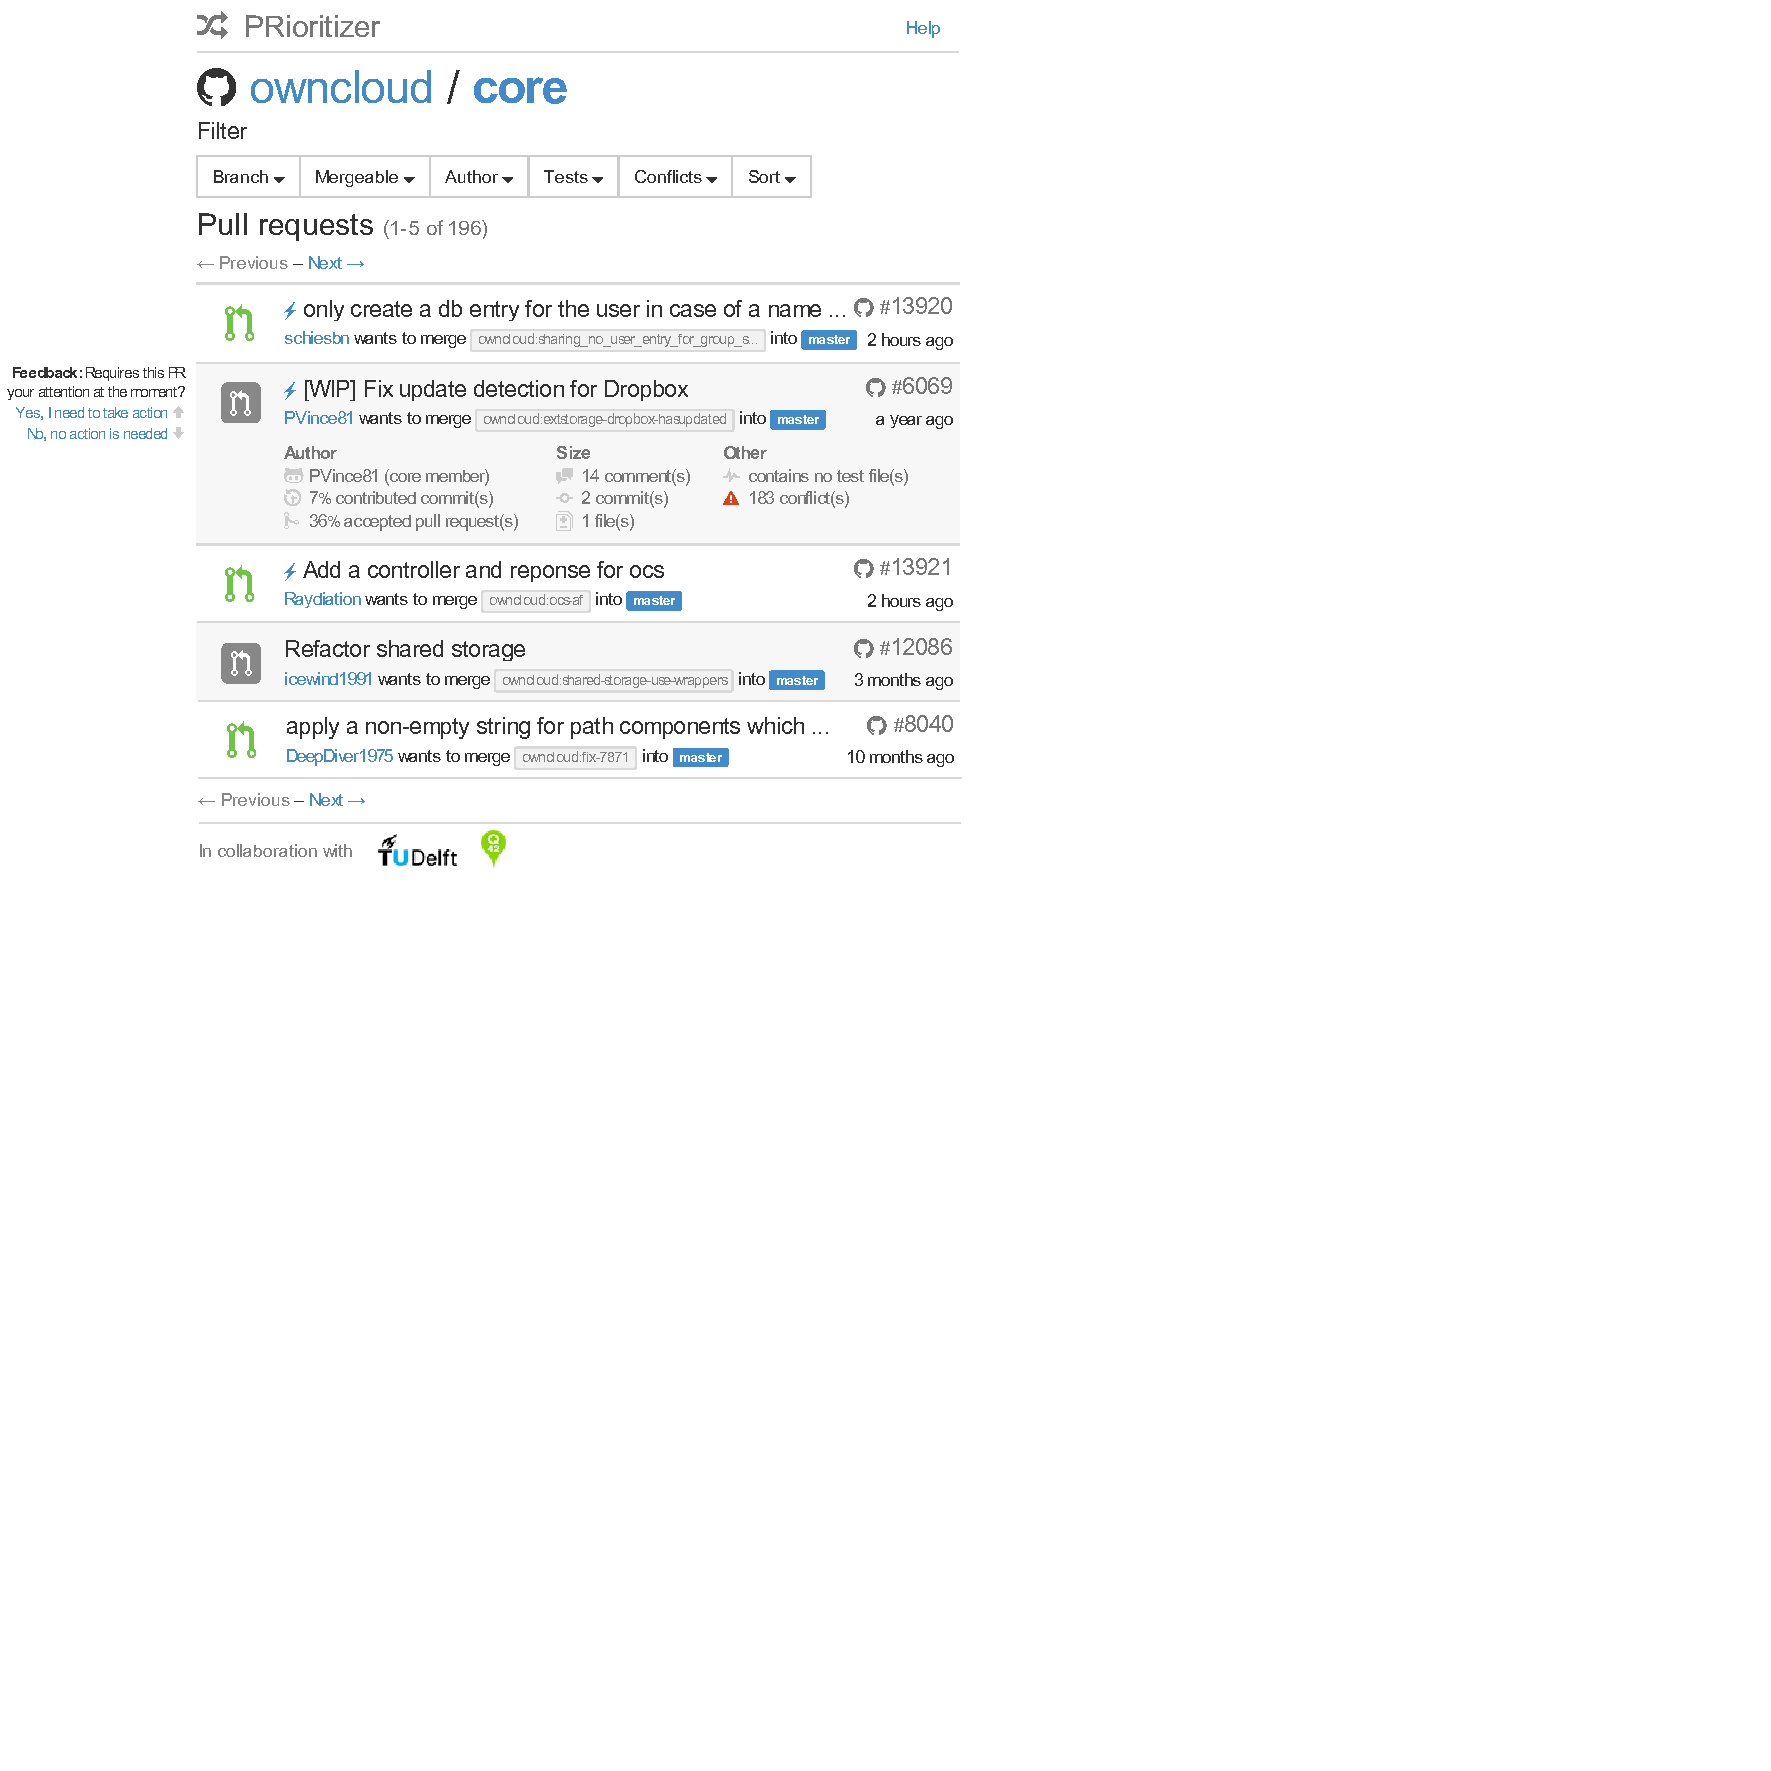
\includegraphics[width=0.5\textwidth]{../figs/interface.pdf}
  \caption[The user interface]
   {The user interface. It shows an ordered list of pull requests that need attention.}
  \label{fig:ui}
\end{figure}

\section{Initial Evaluation}
\label{sec:evaluation}

\subsection{How good are the activity predictions?}
\label{sec:learning}

To select one algorithm to base our prediction engine on, we used historical
data from 475 projects and three commonly used machine learning algorithms:
Logistic Regression, Na\"ive Bayes and Random Forests. The target of the test
was to compare how well models build with each algorithm could predict whether a
pull request would become active in the next time window against the ground
truth.  We ran the three algorithms against each project with a 10-fold random
selection cross-validation. The models were trained with 90\% training data and
10\% testing data.

In table~\ref{tab:alg-compare}, we see how the three algorithms performed. Both
Logistic Regression and Na\"ive Bayes perform badly on precision and accuracy,
which were our top priorities.  On the other hand, Random Forests perform well
over all, even though the recall performance leaves something to be desired. To
improve the performance, we tried several optimisations like dataset balancing
and feature pruning to no avail.

\begin{table}
  \begin{tabular}{lrrrrc}
    \hline
    \textbf{Algorithm} & \textbf{5\%} & \textbf{Mean} & \textbf{Median} & \textbf{95\%} & \textbf{Histogram} \\
    \hline

    \bf{Logistic Regression}\\
    Area Under Curve & 0.71 & 0.81 & 0.81 & 0.91 & 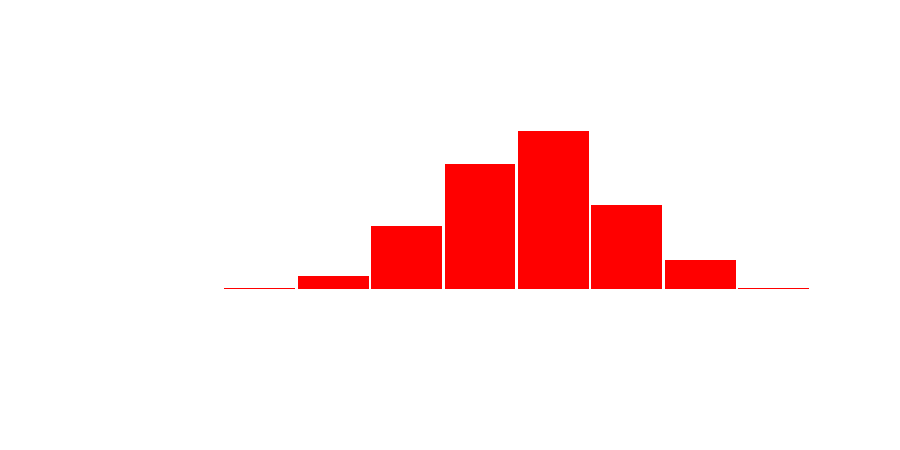
\includegraphics[scale = 0.1, clip = true, trim= 50px 60px 50px 60px]{../figs/hist-results/hist-LRauc.pdf} \\
    Accuracy & 0.52 & 0.62 & 0.62 & 0.72 & 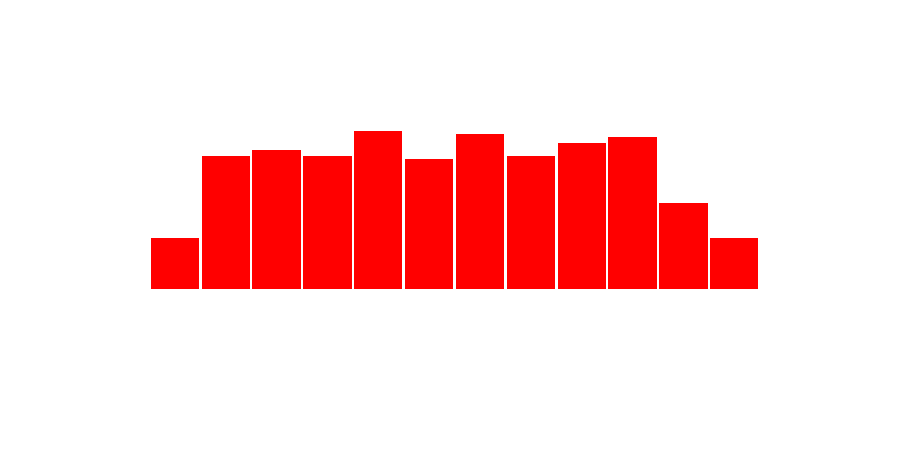
\includegraphics[scale = 0.1, clip = true, trim= 50px 60px 50px 60px]{../figs/hist-results/hist-LRacc.pdf} \\
    Precision & 0.06 & 0.36 & 0.30 & 0.88 & 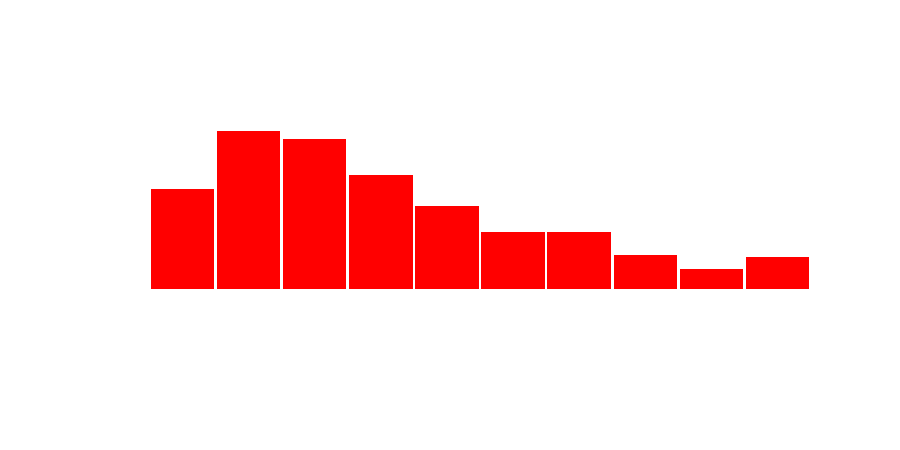
\includegraphics[scale = 0.1, clip = true, trim= 50px 60px 50px 60px]{../figs/hist-results/hist-LRprec.pdf} \\
    Recall & 0.66 & 0.83 & 0.84 & 0.95 & 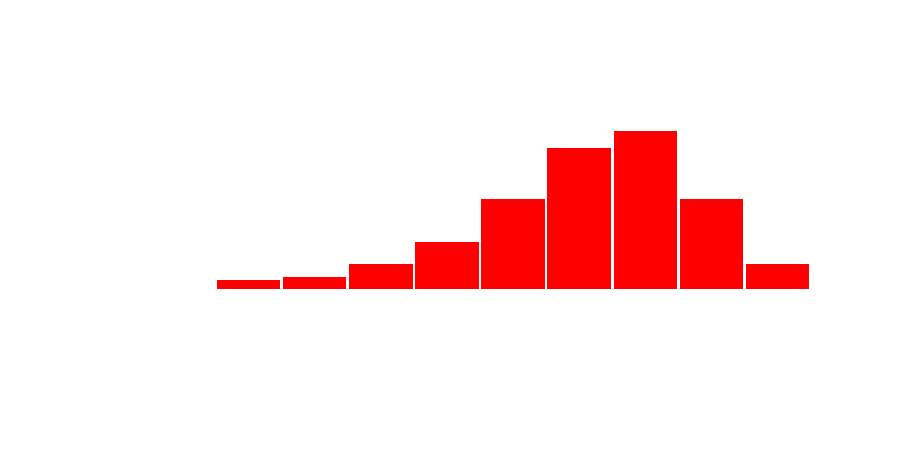
\includegraphics[scale = 0.1, clip = true, trim= 50px 60px 50px 60px]{../figs/hist-results/hist-LRrec.pdf} \\
    F1 & 0.12 & 0.45 & 0.44 & 0.77 & 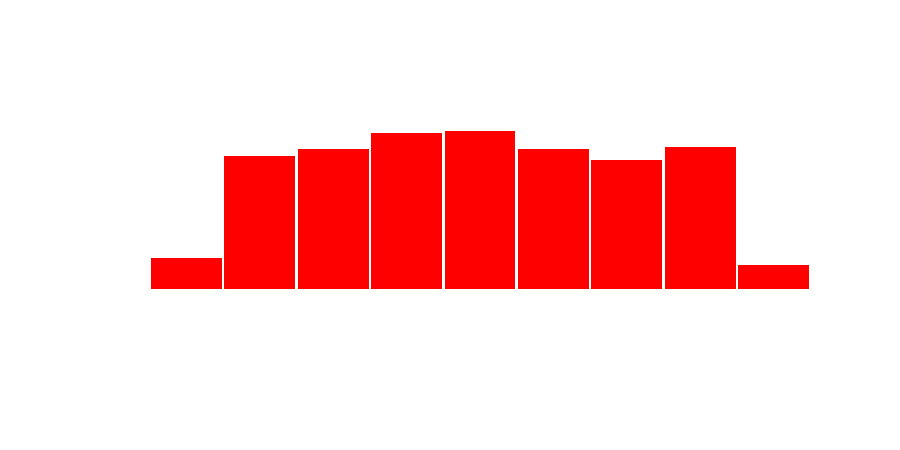
\includegraphics[scale = 0.1, clip = true, trim= 50px 60px 50px 60px]{../figs/hist-results/hist-LRf1.pdf} \\

    \bf{Naive Bayes}\\
    Area Under Curve & 0.65 & 0.75 & 0.75 & 0.86 & 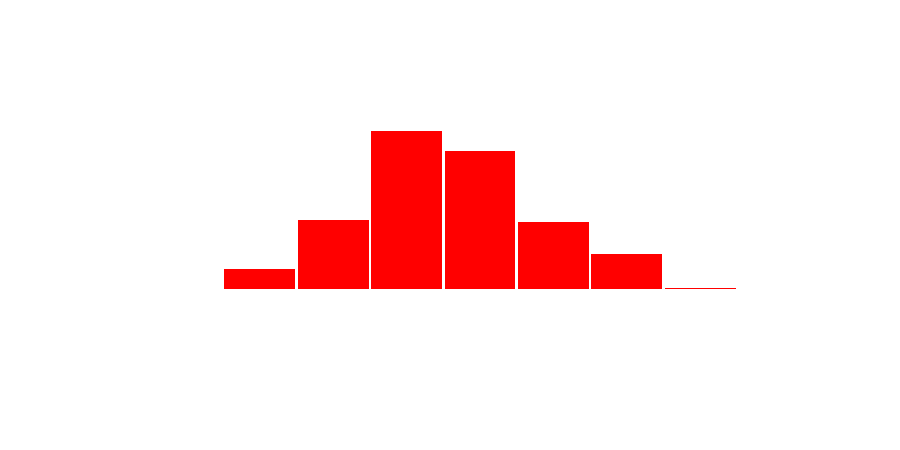
\includegraphics[scale = 0.1, clip = true, trim= 50px 60px 50px 60px]{../figs/hist-results/hist-NBauc.pdf} \\
    Accuracy & 0.52 & 0.60 & 0.60 & 0.69 & 
\includegraphics[scale = 0.1, clip = true, trim= 50px 60px 50px 60px]{../figs/hist-results/hist-NBacc.pdf} \\
    Precision & 0.06 & 0.34 & 0.28 & 0.82 & 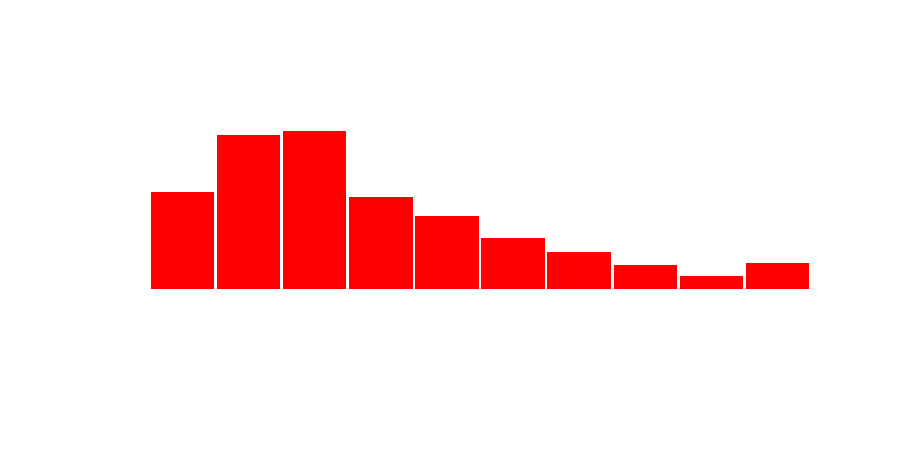
\includegraphics[scale = 0.1, clip = true, trim= 50px 60px 50px 60px]{../figs/hist-results/hist-NBprec.pdf} \\
    Recall & 0.63 & 0.79 & 0.80 & 0.94 & 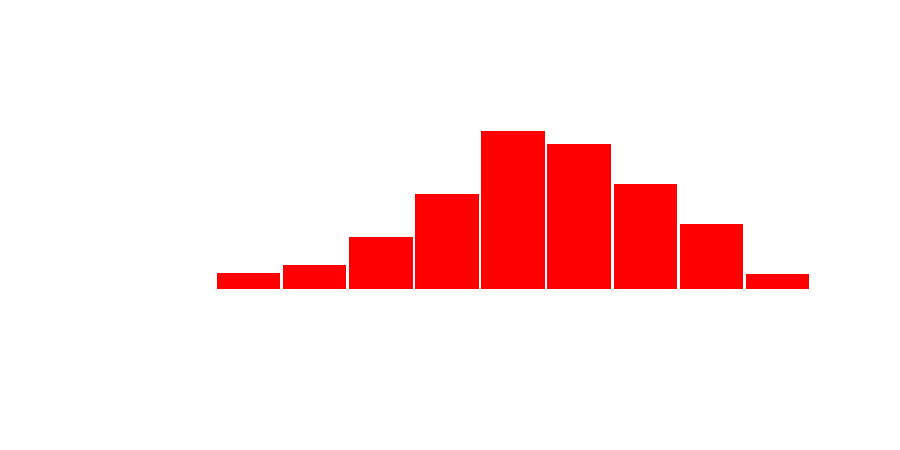
\includegraphics[scale = 0.1, clip = true, trim= 50px 60px 50px 60px]{../figs/hist-results/hist-NBrec.pdf} \\
    F1 & 0.11 & 0.42 & 0.41 & 0.73 & 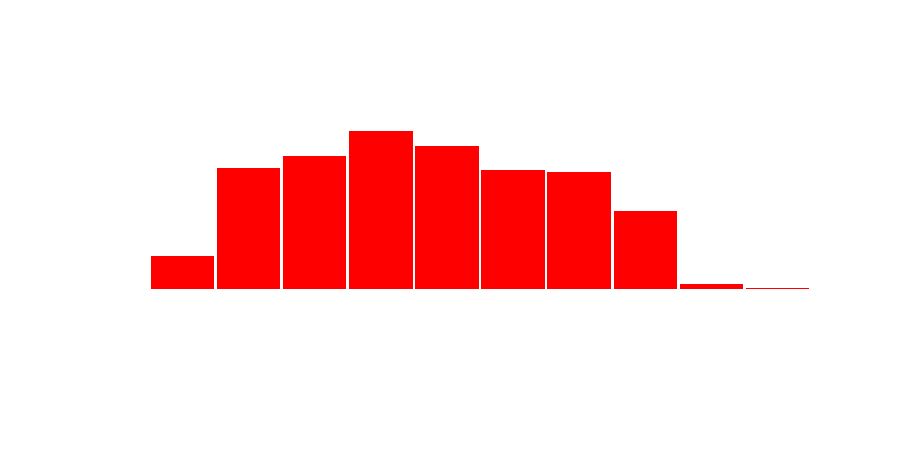
\includegraphics[scale = 0.1, clip = true, trim= 50px 60px 50px 60px]{../figs/hist-results/hist-NBf1.pdf} \\

    \bf{Random Forest}\\
    Area Under Curve & 0.81 & 0.89 & 0.89 & 0.95 & 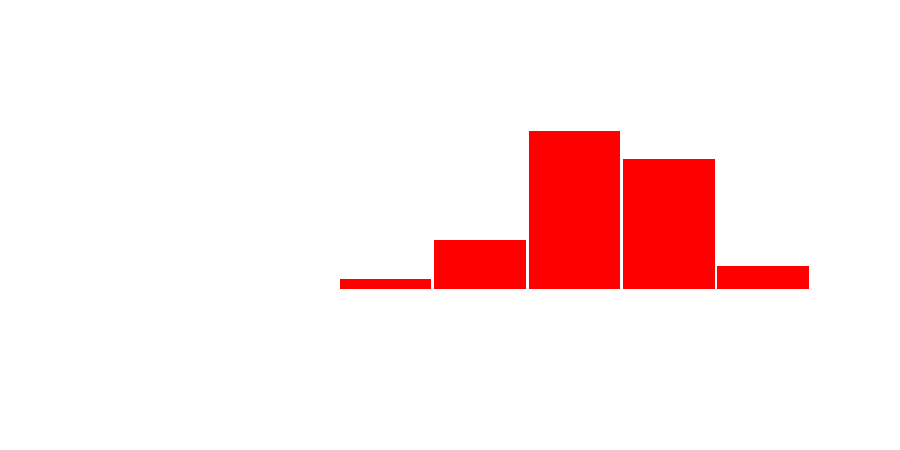
\includegraphics[scale = 0.1, clip = true, trim= 50px 60px 50px 60px]{../figs/hist-results/hist-RFauc.pdf} \\
    Accuracy & 0.73 & 0.86 & 0.87 & 0.96 & 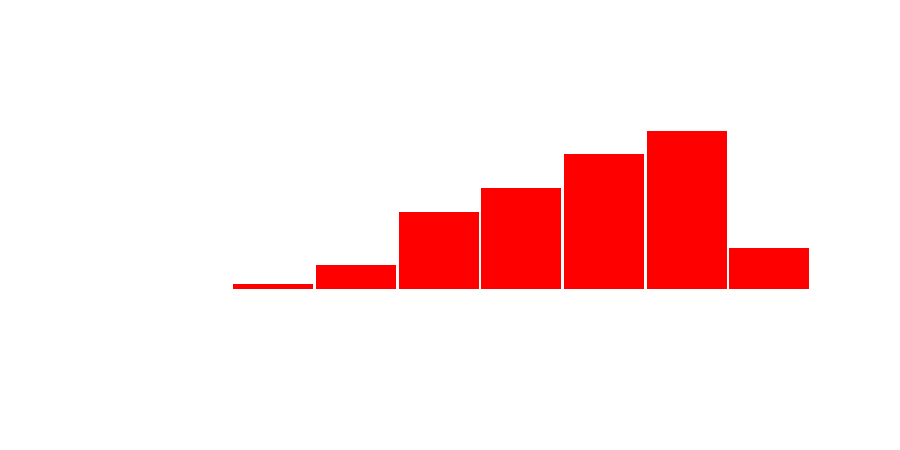
\includegraphics[scale = 0.1, clip = true, trim= 50px 60px 50px 60px]{../figs/hist-results/hist-RFacc.pdf} \\
    Precision & 0.37 & 0.66 & 0.69 & 0.90 & 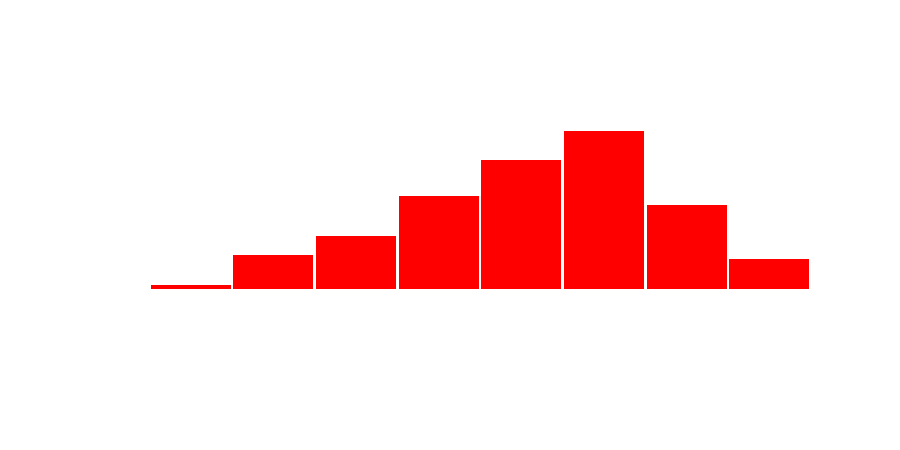
\includegraphics[scale = 0.1, clip = true, trim= 50px 60px 50px 60px]{../figs/hist-results/hist-RFprec.pdf} \\
    Recall & 0.36 & 0.62 & 0.63 & 0.84 & 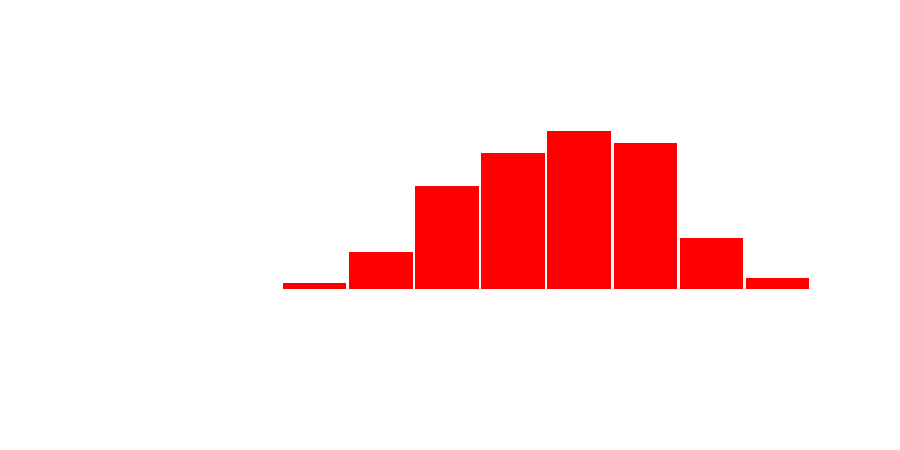
\includegraphics[scale = 0.1, clip = true, trim= 50px 60px 50px 60px]{../figs/hist-results/hist-RFrec.pdf} \\
    F1 & 0.38 & 0.63 & 0.63 & 0.87 & 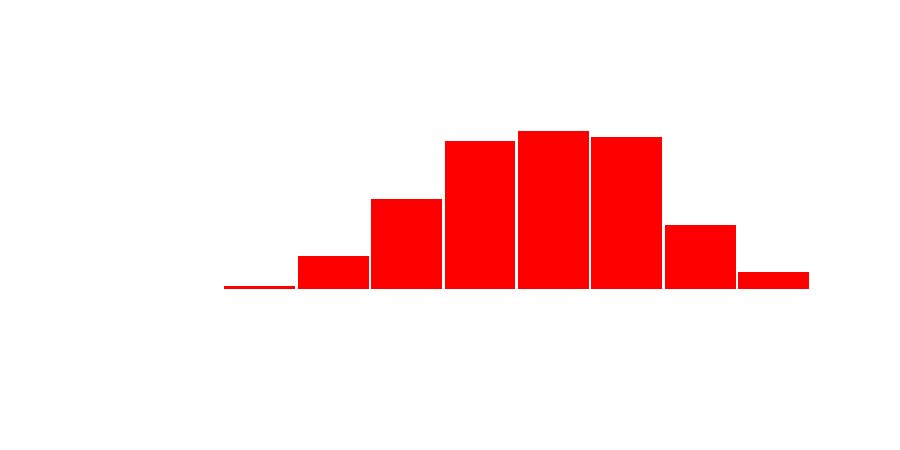
\includegraphics[scale = 0.1, clip = true, trim= 50px 60px 50px 60px]{../figs/hist-results/hist-RFf1.pdf} \\
    \hline
  \end{tabular}
  \caption[Comparision of algorithms]{Scores and distributions of algorithm performance across projects. \erik{As the distributions look fairly normal can you report the mean and standard deviation instead of the median?}}
  \label{tab:alg-compare}
\end{table}

%It is interesting to see that the age is a very dominant factor when we look at
%the feature importance in figure~\ref{fig:feature-importance}.  This is probably
%the case because it is very likely that new pull requests receive comments
%within the first few days.  Since the age feature is so dominant it could impact
%the model in a bad way.  When we turned this particular feature off, the results
%were worse instead.  So it seems the age has a positive effect on the
%prediction.
%
%\begin{figure}
%  \centering
%  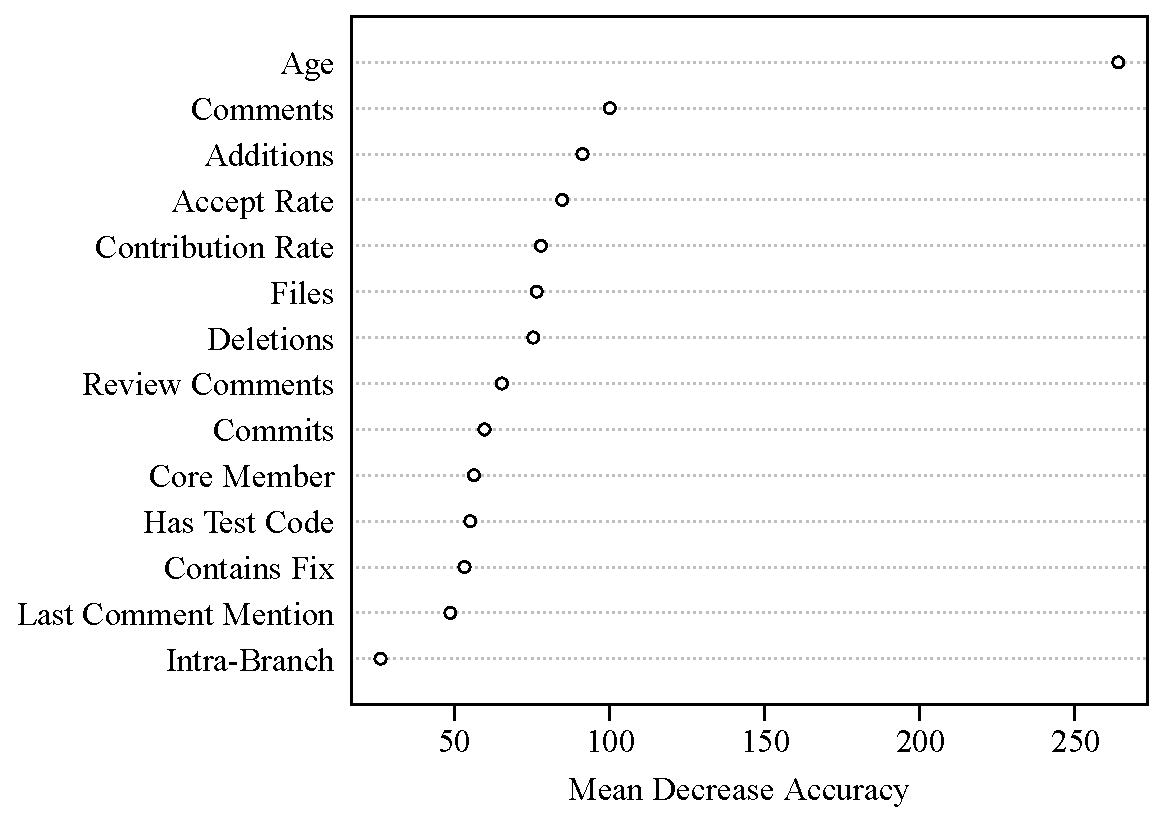
\includegraphics[width=0.45\textwidth]{../figs/mean-decrease-accuracy.pdf}
%  \caption[Plot of feature importance]
%   {Plot of feature importance of the aggregated projects. The age of the pull request is the dominant factor.}
%  \label{fig:feature-importance}
%\end{figure}

The results show that using Random Forests, we can predict with relatively
high accuracy (86\% on average) whether a pull request in a given time frame
of its life will be active in the next one. This is an important result
for building a prioritizer service, as it gives us the confidence to
recommend a default ordering to the service user. Moreover, as the
quality of the prediction varies across projects, we can build preprocessing
phases to determine whether default recommendations can be useful.
However, there is room for improvement: by selecting more representative
features, or custom features for each project, we can account for variations
of pull request handling practices. Moreover, user directed evaluation (already
implemented in the visualizer) can help retrofit our machine learning model
with user preferences.

\subsection{Performance Evaluation}
\erik{Can you provide a couple of paragraphs here? Describe our hardware, the}

\subsection{User Evaluation}

To test our service we invited a group of integrators that maintain open source projects.
The integrators were asked to answer statements on a scale with the following answers: strongly disagree, disagree, agree and strongly agree.
The values to the answers are ${-2, -1, 1, 2}$ respectively.
In addition to analysing their answers directly we also correlate the answers to the activity of their project.
We define the activity of their project as the average number of PR actions per day since the last 6 months.

The first questions were about the usefulness of certain features of the service.
Table~\ref{tab:usefulness} shows the averages of the given answers.
It can be seen that insight in the Contribution Rate, Test Code and Size are the most usefull features.

\resp{5}{The fact you can see how much the author of the pull request did in the past and how his success rate for getting pull requests in.
That is really useful information.
People that have a track record, will have obviously more chance to have their pull request looked at.}

However, the main highlight of the service, the Automatic Ordering, is on average neither positive nor negative rated.
This has probably something to do with the reasons why a certain PR is ranked higher than others (\respnum{6,7,9,17,19,20}).
\resp{17}{It can show us the most pressing pull requests.
However, it is unclear how this ranking is established, so I'd hope to know why a pull request is considered more urgent then others.}

Another thing that can be observed from table~\ref{tab:usefulness} is that the Target Branch and the Pairwise Conflicts features (the manual features) are rated more usefull for projects with more activity.

\begin{table}
  \centering
  \begin{tabular}{lrr}
    \hline
    \textbf{Feature} & \textbf{Average} & \textbf{Activity correlation} \\
    \hline
    Contribution Rate  &  $0.4286$ &  $0.1124$ \\
    Has Test Code      &  $0.3333$ &  $0.0186$ \\
    Size               &  $0.1905$ &  $0.3835$ \\
    Pairwise Conflicts &  $0.0952$ &  $0.4845$ \\
    Automatic Ordering &  $0.0000$ & $-0.0149$ \\
    Target Branch      & $-0.4762$ &  $0.6340$ \\
    Accept Rate        & $-0.0476$ & $-0.2268$ \\
    \hline
  \end{tabular}
  \caption[Usefulness of features]{Usefulness of features. The average usefulness of the features and their correlation with the project activity.}
  \label{tab:usefulness}
\end{table}

The next part is about the usability of the service.
Around 86\% (18) says that using the service causes no extra overhead.
The given answers have a correlation of $0.4441$ with the activity of the project.

76\% (16) of the respondents thinks the prioritized overview of PRs is clear enough.
\resp{1}{I can see at a glance which PRs can be merged automatically.
For some reason the Github PR interface does not show this, you have to click on a PR to find out if it can be automatically merged.
In one of my projects, PRs often sit unmerged for a while and have to be rebased, so it's better to know when rebasing is necessary sooner, rather than later.}

Only 62\% (13) of the respondents agree that the set of used and presented fields is complete.
It seems that the integrators of more active projects tend to disagree, with a correlation of $-0.4054$.
This probably caused by the fact that the prioritization service lacks support for GitHub labels and milestones.

Later on in the questionaire we asked to rate some features for a next version of the prioritization service.
71\% (15) of the respondents indicated that they want to prioritize according to labels.
The correlation between the activity and the lack of label support is $0.4443$.
\resp{7}{I like the autosorting, but I'd like more control over it.
I use labels a lot for things, so for example, `needs followup' is a label that means I need to take no action, so I'd love to be able to tell you that.}

As said earlier, it is not clear for everyone on what grounds one pull request is higher ranked than others.
Almost all respondents (86\% or 18) want more control over the automatic ordering in a future version.
\resp{19}{It's very difficult to tell what the default ordering means.
This might be an inevitable consequence of machine learning but without some insight into why the results were ordered in a certain way (and maybe the ability to tweak the input weights), the view wasn't helpful.}

Finally we asked the respondents if they would use the prioritization service for their project.
57\% (12) of the respondent gave a positive answer.
With a activity correlation of $0.4307$ it seems that integrators with a more active project tend to use it more than those with less active projects.
\resp{15}{I actually don't find it very useful at all.
I've never had a problem prioritising pull requests, we keep the number of open pull requests below 30.
Generally, I respond to all pull requests raised on the project as soon as I receive the notification for them.}

The results are not very conclusive.
It seems that in its current form the automatic ordering is not adequate.
Users want to see why a PR is considered more important than others and have more control over the learning process.
On the other hand the manual sorting and filtering options are positively evaluated.
The Pairwise Conflicts, Target Branch and Size are the most popular.
Although the latter two are fairly trivial features GitHub's interface doesn't support them.
This might be the reason why the are rated useful.
Finally, a narrow majority indicated that they will use the service for their project.

\section{Related Work}

\section{Conclusions and Future Work}

\section*{Acknowledgements} The authors would like to thank Audris Mockus for
fruitful discussions that influenced the design of the prioritization algorithm.

\bibliographystyle{IEEEtran}
\bibliography{prioritizer}


\end{document}
